\icode{E-MI-SI-L2-261107-001}
水平地面上堆放着相同的原木，截面图如图所示，已知原木之间的动摩擦因数为\(\mu\)，每根原木的重力为\(G\)，可将原木看成圆柱体，若要将最上面的那根原木沿轴线方向匀速拉出，水平拉力大小应为\paren[]

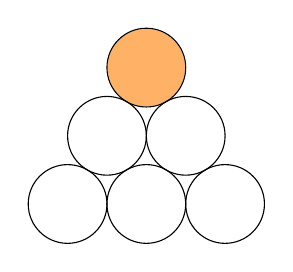
\begin{tikzpicture}[scale=.5]
	\draw[fill=orange!60,draw=white] (0,0) circle(1);
	\foreach \d/\r in {0/0,-120/2,-120/4,-60/2,-60/4}
		\draw (\d:\r) circle(1);
	\draw (-90:{2*sqrt(3)}) circle(1);
\end{tikzpicture}
\begin{choices}
	\item\(\frac{\sqrt{3}}{2}\mu G\)
	\item\(\mu G\)
	\item\(\frac{2\sqrt{3}}{3}\mu G\)
	\item\(2\mu G\)
\end{choices}
\begin{answer}
    
\end{answer}
